%/*% pdflatex -file-line-error -interaction nonstopmode %

\documentclass{article}
\usepackage{graphicx}
\usepackage{amsmath}
\usepackage{amsfonts}
\usepackage{bookmark}
\usepackage{booktabs}
\usepackage{exercises}
\graphicspath{ {./images} }
\usepackage{indentfirst}
\usepackage{amsthm}
\usepackage{yhmath}
\usepackage{placeins}
\newcommand*{\oldneg}{\mathord{\sim}}
\newcommand\showdiv[1]{\overline{\smash{)}#1}}
\newcommand\Mydiv[1]{%
\smash{\raise.3ex\hbox{$\big)$}}\mkern-8mu
        \overline{\enspace\strut#1}}
\setlength{\tabcolsep}{5pt}
\theoremstyle{definition}
\newtheorem{definition}{Definition}

\setlength{\parindent}{.5in}
\setlength{\parskip}{12pt}
\renewcommand{\arraystretch}{1}

\title{2.6 Answers}
\begin{document}
\maketitle

\section*{23}


According to the rational roots theorem, the possible rational zero's of 
\[ f(x)=2x^4-5x^3-10x^2-9 \] are \[ \pm\frac{1}{1},\pm\frac{1}{2},\pm\frac{3}{1},\pm\frac{3}{2},\pm\frac{9}{1},\pm\frac{9}{2} \]
meaning $\frac{5}{2}$ is not a possible zero of the function, and thus the answer is C.

\section*{38}


Take for example the polynomial function:
\[ f(x)=4x^3-2x^2+4x+2 \]
which has the rational zero's:
\[ \pm\frac{1}{1},\pm\frac{2}{1},\pm\frac{1}{2},\pm\frac{2}{2},\pm\frac{1}{4},\pm\frac{2}{4} \]


\section*{40}


Given a leading term $a_n$ that has $r$ factors, and a leading term $a_0$ that has $s$ factors, we know by the rational roots theorem 
that all the possible zero's of $f$ are of the form \[ \dfrac{p}{q} \] where $p$ is a factor of $a_0$ and $q$ is a factor of $a_n$. 
Thus, we are considering $s+r$ objects, and taking $2$ of them at a time, but subtracting from this total $s$ objects taken $2$ at a time
and $r$ objects taken two at a time, as the zeros are only valid if a factor from each of the different coefficients are included. Thus, 
using the formula for $n$ objects taken $r$ at a time, we recieve that the total number of possible zeros is:
\begin{center}
	\begin{tabular}{lll}
		& $\dfrac{(s+r)!}{((s+r)-2)!\times 2!}-\dfrac{r!}{(r-2)!\times 2!}-\dfrac{s!}{(s-2)!\times 2!}$ \\
		= & $\dfrac{(s+r)!}{((s+r)-2)!\times 2}-\dfrac{r!}{(r-2)!\times 2}-\dfrac{s!}{(s-2)!\times 2}$ & Because $(2!=2)$ \\
		= & $\dfrac{(s+r)(s+r-1)}{2}-\dfrac{r(r-1)}{2}-\dfrac{s(s-1)}{2}$ & Because $\dfrac{n!}{(n-2)!}=n(n-1)$ \\
		= & $\dfrac{(s+r)(s+r-1)-r(r-1)-s(s-1)}{2}$ \\
		= & $\dfrac{(s^2+r^2+2rs-s-r)-(r^2-r)-(s^2-s)}{2}$ \\
		= & $\dfrac{2rs}{2}$ \\
		= & $rs$
	\end{tabular}
\end{center}
thus meaning the amount of possible real zero's is equal to $rs$.
	 

\section*{45}
We are given a rectangular prism with a square base. We are given that the height is $x+4$ inches, where $x$ is the length of the square
base. We also know that the volume is $63$ cubic inches, meaning we have the following equation:
\[ 63=(x+4)x^2 \]
\[ 63=x^3+4x^2 \]
\[ x^3+4x^2-63=0 \]
By the rational roots theorem, we know that the possible solutions to the equation are:
\[ \pm\frac{1}{1},\pm\frac{3}{1},\pm\frac{7}{1},\pm\frac{9}{1},\pm\frac{21}{1},\pm\frac{63}{1} \]
Using a calculator, one can check all of these solutions, and can determine that $3$ is the only rational solution. 
Thus, the dimensions of the 
pool are $3+4=7$ inches high by $3$ feet wide by $3$ feet long.

\section*{48}
\setlength{\tabcolsep}{10pt}
We are given a pyramid having a square base with side lengths of $x$, a height of $2x-5$, and a volume of $3$. Recall that the 
volume of a pyramid is given by:
\[ V=\frac{1}{3}bh \] meaning the equation in this case is:
\[ 3=\frac{1}{3}x^2(2x-5) \]
\[ 9=x^2(2x-5) \]
\[ 9=2x^3-5x^2 \]
\[ 2x^3-5x^2-9=0 \]
By the rational roots theorem, the possible rational roots of this equation are:
\[ \pm\frac{1}{1},\pm\frac{3}{1},\pm\frac{9}{1},\pm\frac{3}{2},\pm\frac{9}{2} \]
Using a calculator, one can check all of these solutions, and can determine that $3$ is a solution. By the factor theorem, 
$x-3$ is a factor of this function, meaning we can use synthetic division to find the other factor:
\FloatBarrier
\begin{center}
	\begin{tabular}{l|rrrr}
		$3$ & $2$ & $-5$ & $0$ & $-9$ \\
		& & $6$ & $3$ & $9$ \\
		\cmidrule{2-5}
		& $2$ & $1$ & $3$ & $0$
	\end{tabular}
\end{center}
\FloatBarrier
meaning the other factor is \[ 2x^2+x+3 \] because \[ b^2-4ac=1^2-4(2)(3)=-23<0 \] we know that the solutions to this equation are both 
imaginary, meaning the only possible real solution is $x=3$. Thus, the dimensions of the pyramid are $3$ ft. wide by $3$ ft. long by 
$2(3)-5=1$ ft. high. 

\section*{49}
We are given that from 1994 to 2003, the amount of athletic equipment $E$ (in millions of dollars) sold domestically can be modeled by
\[ E(t)=-10t^3+140t^2-20t+18,150 \]
where $t$ is the number of years since 1994. We are aksed to find the year when about $\$20,300,000,000$ of athletic equipment 
was sold.\newline
(a): Because the equations takes the sale in millions of dollars, we can write this equation as:
\[ 20300=-10t^3+140t^2-20t+18150 \]
\[ 20300=10(-t^3+14t^2-2t+1815) \]
\[ 2030=-t^3+14t^2-2t+1815 \]
\[ -t^3+14t^2-2t-215=0 \]
(b): The only whole number (and positive) possible solutions from part (a) less than 10 are \[ \frac{1}{1},\frac{5}{1} \]
(c): Using a calculator, we can see that $x=5$ is the only such solution. This means that the year that corresponds to the solution is 
\[ 1994+5=1999 \] 

\section*{50}
We are given that, since $1990$, the number of U.S. travelers to foreign countries $F$ (in thousands) can be modeled by 
\[ F(t)=12t^4-264t^3+2028t^2-3924t+43916 \]
where $t$ is the number of years since 1990. We are aksed to find the year when there were about 56,300,000 travelers.\newline
(a): Because the equation takes the number of travelers in the thousands, we can write this equation as:
\[ 56300=12t^4-264t^3+2028t^2-3924t+43916 \]
\[ 0=12t^4-264t^3+2028t^2-3924t-12384 \]
\[ 0=12(t^4-22t^3+169t^2-327t-1032) \]
\[ t^4-22t^3+169t^2-327t-1032=0 \]
(b): By the rational roots theorem, the possible solutions that are less than or equal to ten (and $>0$) are the following:
\[ \frac{1}{1},\frac{2}{1},\frac{3}{1},\frac{4}{1},\frac{6}{1},\frac{8}{1} \]
(c): Using synthetic division, we can see that $x=8$ is the only rational solution:
\FloatBarrier
\begin{center}
	\begin{tabular}{l|rrrrr}
		$8$ & $1$ & $-22$ & $169$ & $-327$ & $-1032$ \\
		& & $8$ & $-112$ & $456$ & $1032$ \\
		\cmidrule{2-6}
		& $1$ & $-14$ & $57$ & $129$ & $0$
	\end{tabular}
\end{center}
\FloatBarrier
(d): 
\FloatBarrier
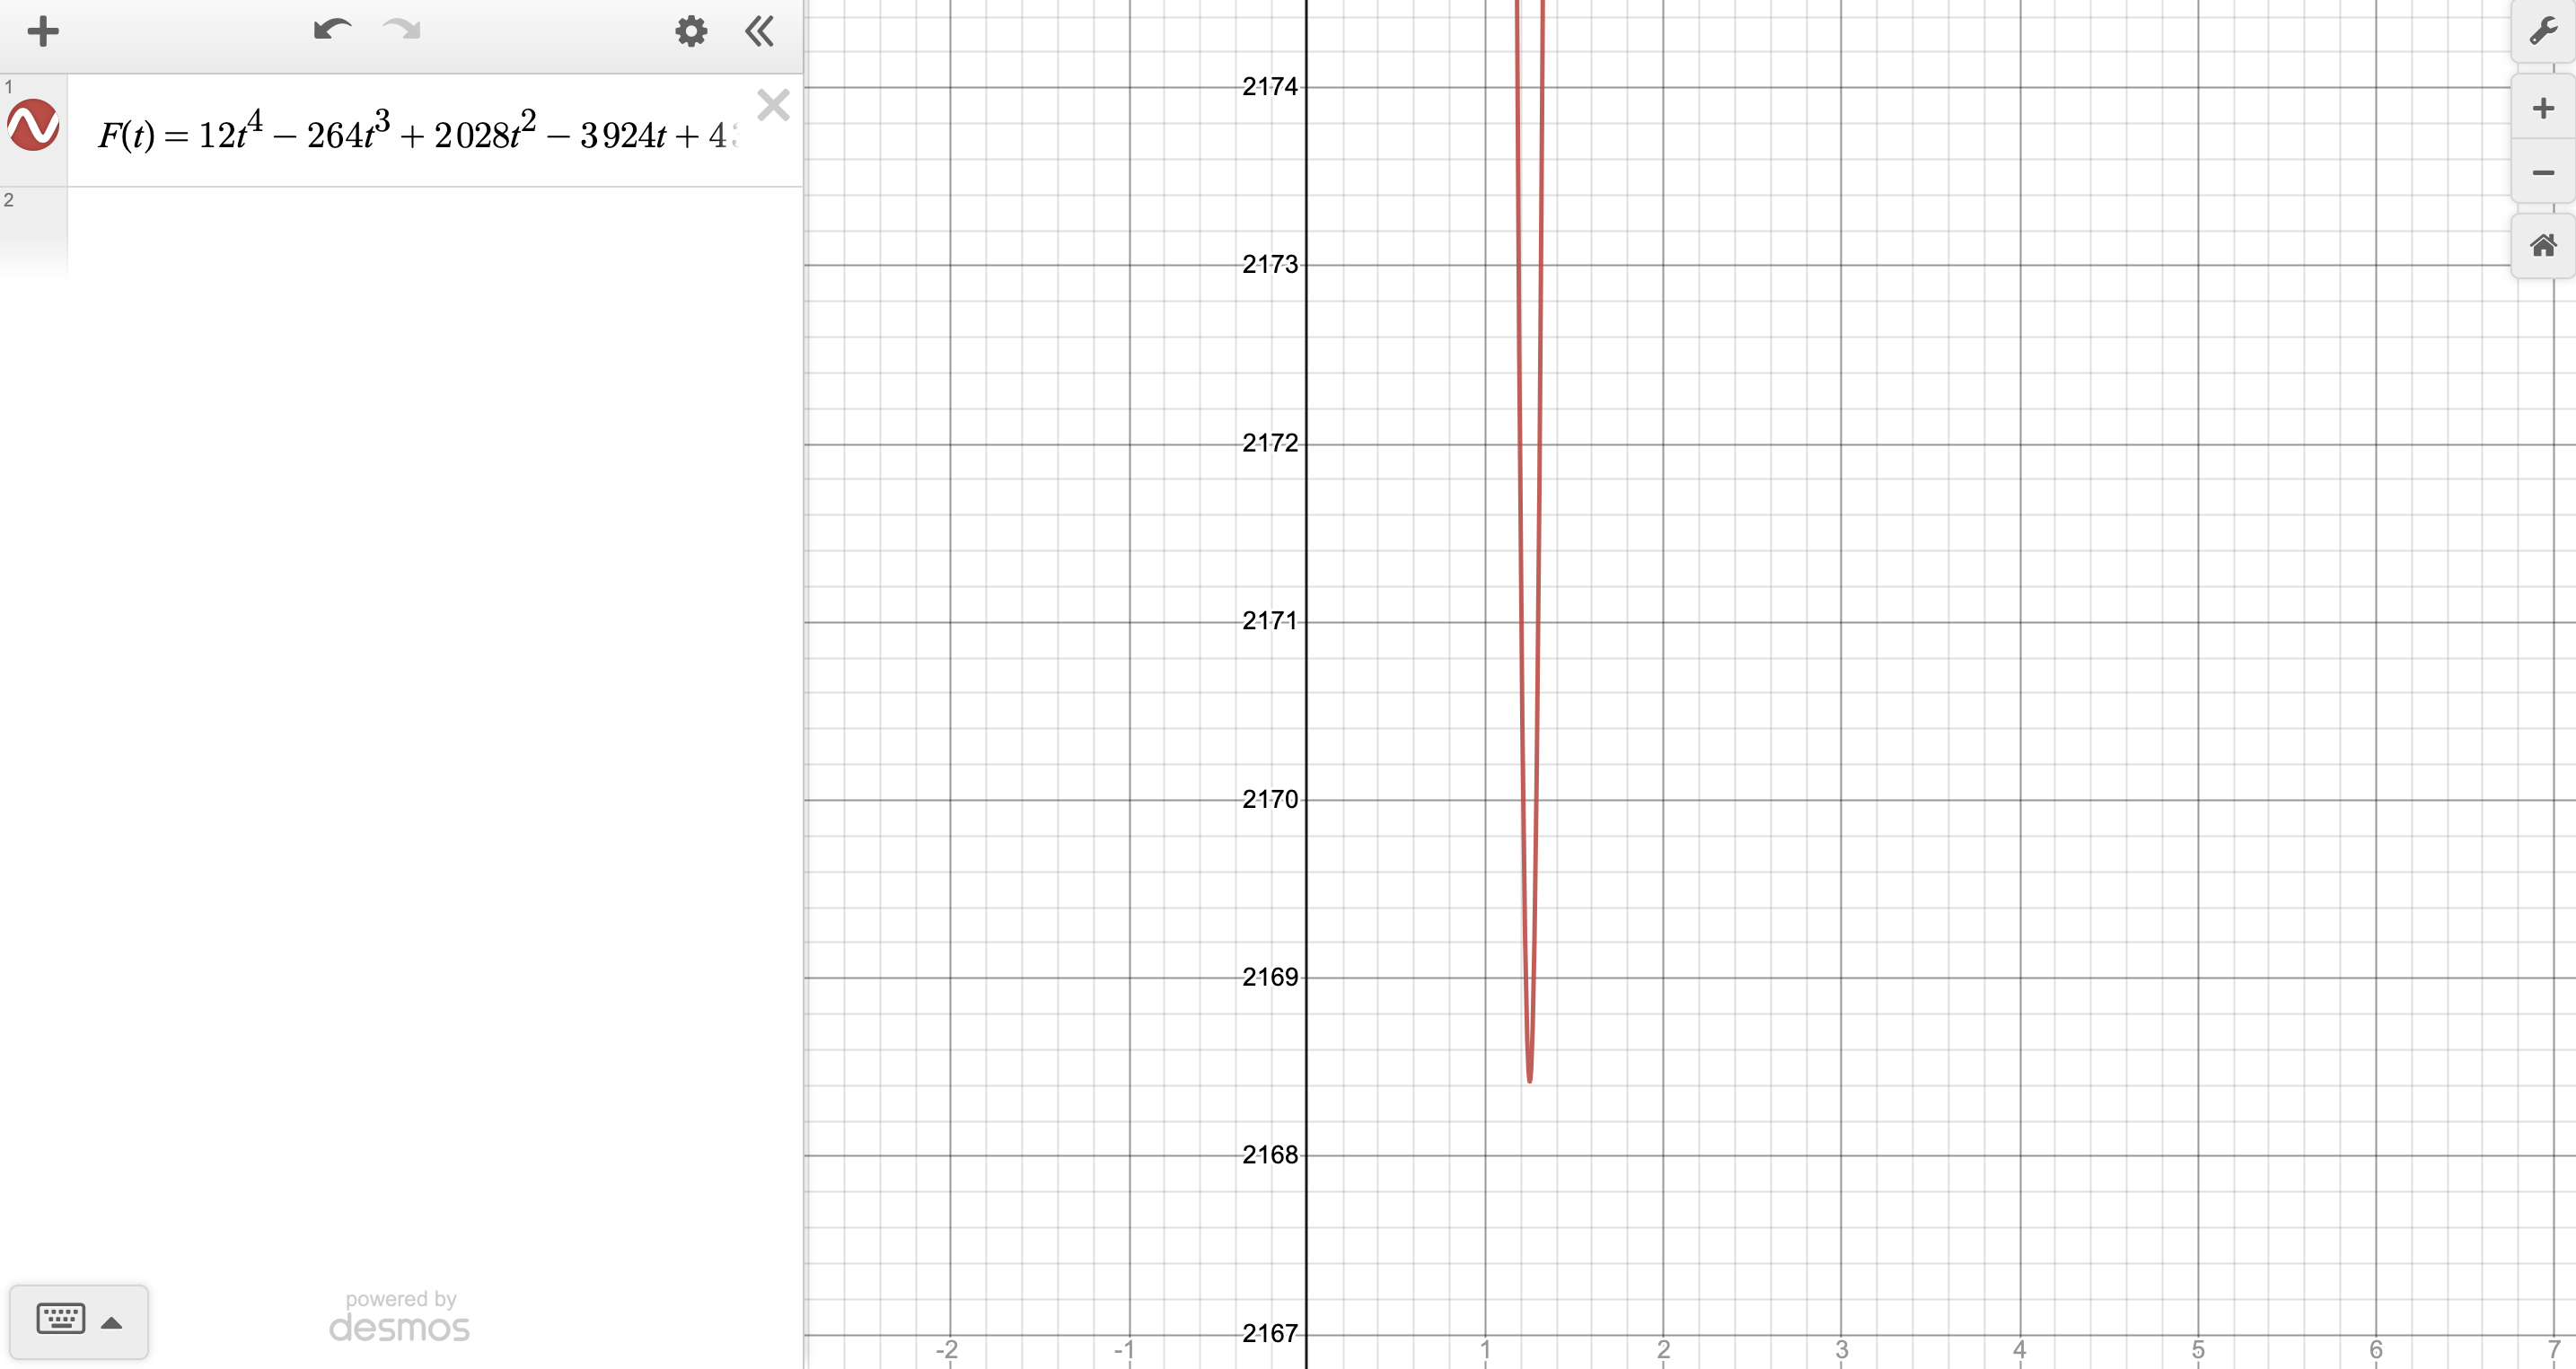
\includegraphics[width = 4in, height = 4in]{2.6picture1}
\FloatBarrier
because we know that $8$ is a solution of the function, we know by the factor theorem that it is also a factor of the same function. 
Thus, we can use synthetic division to find the other factor. Looking back to part (c), this means we have found out that the other factor 
is \[ x^3-14x^2+57x+129 \]
We then consider the equation \[ x^3-14x^2+57x+129=0 \]
By the rational roots theorem, the possible rational roots of this equation are:
\[ \pm\frac{1}{1},\pm\frac{3}{1},\pm\frac{43}{1},\pm\frac{129}{1} \]
Using a calculator, one can see that none of these possible solutions are actually solutions, meaning this equation has no 
rational solutions. Thus, $x=8$ is the only rational solution, meaning it is the only possible solution for this problem. Thus, the year 
when there were about $56,300,000$ travelers was in \[ 1990+8=1998 \]

\section*{51}
We are given a pair of ramps. We know that the length between the two ramps is $3x$, and the height of the two ramps is $x$, while 
their widths are both $3x$. We are given a length from the end of one ramp to the end of the other, with space in between; this 
length is $21x+6$. We know that 
the space in between is $3x$, meaning the combined length of the two ramps is $21x+6-3x=18x+6$. Also, we are given that the left ramp 
is twice as long as the right ramp, meaning we have the following equation for $y$, the length of the left ramp:
\[ y+\frac{1}{2}y=18x+6 \]
\[ \frac{3}{2}y=18x+6 \]
\[ y=12x+4 \]
meaning the length of the left ramp is $12x+4$, while the length of the right ramp is $6x+2$. Thus, the dimensions for the left ramp are 
\[ 12x+4\textrm{ ft. long by } 3x\textrm{ ft. wide by } x\textrm{ ft. high } \]
while the dimensions for the right ramp are
\[ 6x+2\textrm{ ft. long by } 3x\textrm{ ft. wide by } x\textrm{ ft. high } \]
We are given that the total volume of concrete required to build the two ramps is $150$ cubic feet. We know that each ramp is just half 
of the rectangular prisms with their corresponding measurements, meaning we have the following equation:
\[ 150=\frac{1}{2}(12x+4)(3x)x+\frac{1}{2}(6x+2)(3x)x \]
\[ 150=\frac{1}{2}(36x^3+12x^2)+\frac{1}{2}(18x^3+6x^2) \]
\[ 150=(18x^3+6x^2)+(9x^3+3x^2) \]
\[ 27x^3+9x^2-150=0 \]
\[ 9x^3+3x^2-50=0 \]
We can then use the rational roots theorem to determine the possible real number solutions:
\[ \pm\frac{1}{1},\pm\frac{1}{3},\pm\frac{1}{9},\pm\frac{2}{1},\pm\frac{2}{3},\pm\frac{2}{9},\pm\frac{5}{1},\pm\frac{5}{3},\pm\frac{5}{9}, \]
\[ \pm\frac{10}{1},\pm\frac{10}{3},\pm\frac{10}{9},\pm\frac{25}{1},\pm\frac{25}{3},\pm\frac{25}{9},\pm\frac{50}{1},\pm\frac{50}{3}, \]
\[ \pm\frac{50}{9} \]
using a calculator, one can determine that $\frac{5}{3}$ is one such solution. 
By the factor theorem, this means that $x-\frac{5}{3}$ is a factor of $9x^3+3x^2-50$. We can use synthetic division to find the other factor:
\FloatBarrier
\begin{center}
	\begin{tabular}{l|rrrr}
		$\frac{5}{3}$ & $9$ & $3$ & $0$ & $-50$ \\
		& & $15$ & $30$ & $50$ \\
		\cmidrule{2-5}
		& $9$ & $18$ & $30$ & $0$
	\end{tabular}
\end{center}
\FloatBarrier
meaning the other factor is $9x^2+18x+30$. Because
\[ b^2-4ac=18^2-4(9)(30)=-756<0 \] both of the solutions to this equation are imaginary, meaning $x=\frac{5}{3}$ is the only possible 
measurement. 
We can then conclude that $x=\frac{5}{3}$, meaning 
the dimensions of the left ramp are:
\[ 12(\frac{5}{3})+4=24\textrm{ ft. long by } 5\textrm{ ft. wide by } \frac{5}{3}\textrm{ ft. high } \]
while the dimensions of the right ramp are:
\[ 6(\frac{5}{3})+2=12\textrm{ ft. long by } 5\textrm{ ft. wide by } \frac{5}{3}\textrm{ ft. high } \]
\end{document}
